\section{Introduction}
A long-term goal of robotics research is the introduction of intelligent household robots.
To be effective, such robots will need to perform complex tasks (e.g., setting a dinner table, doing laundry)
over long horizons. Planning for these long-horizon tasks is infeasible
for state-of-the-art motion planners, making the need
for a hierarchical system of reasoning apparent.

One way to approach hierarchical planning is through combined \emph{task and motion planning} (TAMP). In this
approach, an agent is given a symbolic, logical characterization of actions (e.g., move, grasp,
putdown), along with a geometric encoding of the environment. The hierarchical separation of high-level, symbolic task planning
from low-level, geometric motion planning enforces abstraction:
the task planner maintains no knowledge of the environment geometry, and the
motion planner has no understanding of the overall goal.
Efficient integration of these two types of reasoning is challenging, and recent research has
proposed several methods for it~\cite{srivastava2014combined, kaelbling2011hierarchical,
lagriffoul2014orientation, GarrettWAFR14, dornhege2012semantic}.

\begin{figure}[t]
  \centering
    \noindent
    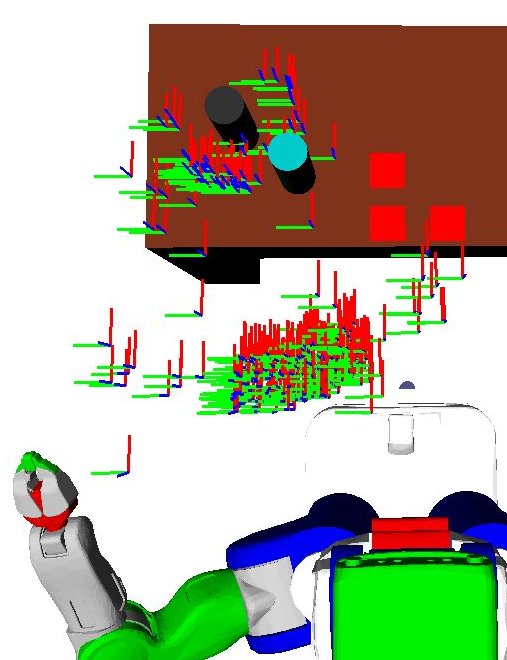
\includegraphics[scale=0.2]{images/move_grasp.png}\hspace{10 mm}
    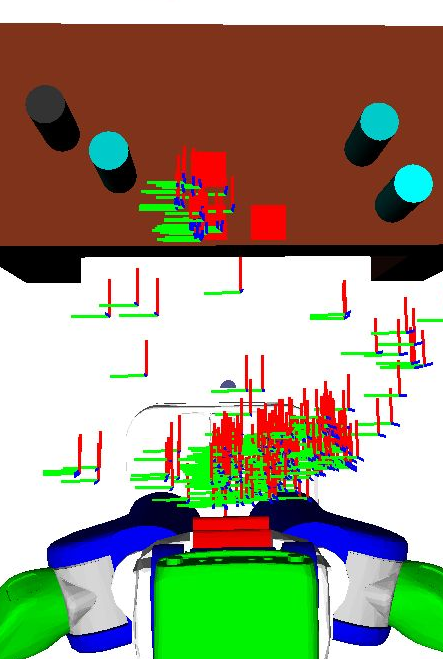
\includegraphics[scale=0.2]{images/move_putdown.png}
  \caption{Screenshots showing some distributions learned by our system in a simulated pick-and-place
    domain. We use reinforcement learning to train good sampling distributions for continuous motion
    planning parameters in long-horizon tasks. The robot is tasked with grasping the black cylinder and putting it down on the
    central red square. The left image shows learned base motion (blue) and grasping (green) distributions,
    and the right shows learned base motion (blue) and putdown (green) distributions. The grasping policy
    learned automatically to avoid the region close to the light blue obstruction. These distributions are
    optimized to reduce the number of motion planner calls needed to produce a complete plan.}
  \label{fig:cover}
\end{figure}

A key limitation of TAMP systems is that they typically rely on hand-coded discretization when
sampling continuous parameter values, such as target grasp poses, for motion planning.
Designing these heuristic sampling distributions often requires substantial effort, as it necessitates
a parametrization of the trajectories a robot must follow to perform actions in its environment.
Often, these parametrizations are tuned based on geometric attributes of the environment and its objects,
meaning that they must be recalibrated when running the system in a new setting. Further,
such discretizations must be fairly coarse to allow reasonable search speeds, meaning they inherently lack
robustness to increased environmental complexity. In this paper, we present a reinforcement
learning method to train good proposal distributions for sampling continuous parameter
values intelligently. The distributions we learn are not discrete, and they implicitly parametrize feasible
robot trajectories. We also develop a method for making the meta-level decision of which
symbolic task sequence to sample for, given options that stem from several potential logical
states of the world.

Our solution builds on the TAMP system
presented by Srivastava et al.~\cite{srivastava2014combined}.
In this system, a (classical) task planner produces a symbolic plan containing
a sequence of actions to reach a goal state. Then, in a process known as \emph{plan refinement},
candidate values are proposed for the continuous variables in this symbolic plan, thus grounding it.
These candidate values are checked locally for feasibility by calling a motion planner.

The authors propose an \emph{interface layer} for refining the plan into a set
of collision-free trajectories; it performs an exhaustive
backtracking search over a hand-coded discrete set of candidate parameter values. If a motion
planning feasible refinement is not found within the resource limit,
symbolic error information is propagated back to the task planner, and a new symbolic plan is produced.
This plan is added as a child node in the \emph{plan refinement graph}, whose nodes store each
symbolic plan and associated current refinement. The search policy through this graph determines the order
in which plans are attempted to be refined. The system uses an off-the-shelf classical task planner and motion planner, both as black boxes.
While our method is specific to this architecture, it can be adapted for other TAMP paradigms.

Reinforcement learning (RL) refers to the process of an agent learning a policy (a mapping from states to actions)
in its environment that maximizes rewards. Zhang and Dietterich~\cite{JobShopSched} first applied the RL framework
to planning problems, using a job shop scheduling setting. In this work, we take inspiration from
their approach; we apply RL to plan refinement in a TAMP system. We implement our approach using methods adapted from
Zucker et al.~\cite{workspacebias}, who train a configuration space sampler for motion planning
using features of the discretized workspace. We train a policy that
determines how to sample values for plan refinement, using policy optimization with linear function
approximation. Our approach allows the learned distributions to be continuous, robust to changes in
the environment, and trainable for any experimental setting, eliminating the need for hand-tuned
distribution parameters. We also train heuristics that encode a search policy through a plan refinement graph.

The four contributions of our work are as follows: 1) we present randomized refinement, a local search
algorithm for plan refinement that is easily formulable as an MDP; 2) we formulate plan refinement in the
RL framework and learn a policy for this MDP; 3) we train heuristics to search intelligently
through a plan refinement graph, allowing us to decide \emph{which} plan to refine next;
and 4) we present experiments to evaluate our approach in a variety of simulated
domains. Our experimental results demonstrate that our approach yields significantly improved
performance over that of hand-coded discretization of the plan refinement sample space.
